% Chapter Template

\chapter{Simulation Physics} % Main chapter title

\label{ch:models} % Change X to a consecutive number; for referencing this chapter elsewhere, use \ref{ChapterX}

\lhead{Chapter 2. \emph{Simulation Physics}} % Change X to a consecutive number; this is for the header on each page - perhaps a shortened title

%----------------------------------------------------------------------------------------
%	SECTION 1
%----------------------------------------------------------------------------------------

\section{Simulations Used}
To demonstrate the efficacy of the various uncertainty quantification methods we use in this work, we employ
several independent simulations (hereafter referred to as ``codes'') of increasing complexity.  These codes
range from simple polynomial evaluations to analytic solutions of simple physics, to nonlinear multistage
iterative solvers representing complex codes.  We describe each briefly here.

\section{Polynomial Evaluations}
In order to benchmark the simplest cases, we make use of simple polynomial expressions of the form
\begin{equation}
  u(Y) = \prod_{i=1}^N (y^b_i+a),
\end{equation}
where $u(Y)$ is the quantity of interest, $Y=[y_1,y_2,\ldots,y_N]$ is the vector of uncertain inputs, and $a$
and $b$ are arbitrary scalar values.  The input variables $Y$ can be distributed arbitrarily.
These polynomials are demonstrations where SCgPC evaluates exactly at some
finite expansion level.




\section{Attenuation}
To demonstrate the convergence rates of various methods, we make use of an adjusted attenuation problem that
is equivalent to the penetration of point particles in a purely-absorbing medium.  The uncertain input
variables are each the length of a segment of material, and each segment has an identical cross section equal
to 1.  The quantity of
interest is the percentage of particles exiting the material.  We normalize the length of the segments to
preserve significant values for the percentage exiting.  The solution to this problem is
\begin{align}
  u(Y) &= \prod_{i=1}^N e^{-Y_i/L},\\
  u(Y) &= \sum_{i=1}^N \exp\left[\frac{\sum_{i=1}^N -Y_i}{L}\right],
\end{align}
where $L=|Y|_1$ is the total segment length.  The input variables $Y$ can be distributed arbitrarily.

The benefit of this model is a simple analytic solution, which makes analytic benchmarks possible.  In
addition, because of the exponential form, SCgPC will converge on a solution, but not replicate it exactly as
in the polynomial case.  This allows accurate comparison between MC, SCgPC methods, and HDMR methods.




\section{Projectile}
For a nonlinear case without an analytic solution, we consider the path traveled by a projectile near the
surface of the Earth, considering varying gravitational pull with height as well as drag on the projectile
from stagnant air.  The equations governing travel in both vertical position $x$ and horizontal position $y$
are given by
\begin{equation}
  y(t) = \frac{v_T}{g}(v\sin\theta+v_T)\left(1-\exp\left[\frac{-gt}{v_T}\right]\right)-v_T t,
\end{equation}
\begin{equation}
  x(t) = \frac{vv_T\cos\theta}{g}\left(1-\exp\left[\frac{-gt}{v_T}\right]\right),
\end{equation}
where $t$ is time, $g$ is acceleration due to gravity, $v$ is scalar velocity, $\theta$ the angle between the
velocity vector and the horizontal ground, $v_T=\frac{mg}{D}$ is terminal velocity, $D=\frac{\rho CA}{2}$ is
the acceleration due to drag, $C$ is the drag coefficient, and $A=\pi r^2$
is the surface area of the projectile in the direction of travel.  The projectile is assumed to present an
identical surface area in both $x$ and $y$ directions.  The quantity of interest is the range, or the total
distance in $x$ traveled by the ball before reaching a height of $y=0$.  The uncertain input variables are
distributed uniformly as described in Table \ref{tab:proj dist}.

\begin{table}[h]
\centering
\begin{tabular}{c | l | c c | c}
  Variable & Name & Mean & Range ($\pm$) & Units \\\hline
  $y_i$ & Initial Height & 1 & 1 & m\\
  $v$ & Initial Velocity & 35.5 & 2.5 & m/s\\
  $\theta$ & Initial Angle & 45 & 10 & degrees\\
  $g$ & Accel. Gravity & 9.79888 & 0.0349 & m/s/s\\
  $m$ & Projectile Mass & 0.145 & 0.0725 & kg\\
  $r$ & Projectile Radius & 0.0336 & 0.00336 & m\\
  $C$ & Drag Coefficient & 0.5 & 0.5 & \\
  $\rho$ & Air Density & 1.2 & 0.1 & kg/m$^3$ \\
\end{tabular}
\caption{Projectile Problem Distributions}
\label{tab:proj dist}
\end{table}

This simulation has the benefit of an analytic solution when $C=0$ and eight distinct input parameters of
varying importance.  This is especially useful in considering anisotropic treatment of the input space.




\section{Neutron Diffusion}
For a nonlinear system with complicated physics, we consider a two-group, two-dimensional neutron diffusion
criticality calculation.  We make use of the diffusion approximation for neutron transport, which provides us
with a coupled set of elliptic PDEs to solve:
\begin{equation}
-\grad\cdot\qty( D_1(\bar x)\grad\phi_1(\bar x))+\qty(\xs{a}{1}(\bar x)+\xs{s}{1\to2}(\bar x))\phi_1(\bar x) = \frac{1}{k(\phi)}\sum_{g'=1}^2\nu_{g'}\xs{f}{g'}(\bar x)\phi_{g'}(\bar x),
\end{equation}
\begin{equation}
-\grad \cdot\qty(D_2(\bar x)\grad \phi_2(\bar x))+\xs{a}{2}(\bar x)\phi_2(\bar x) = \xs{s}{1\to 2}(\bar x)\phi_1(\bar x),
\end{equation}
where we use the following parametric coefficients: the absorption cross section
$\Sigma_{g,a}=\Sigma_{g,c}+\Sigma_{g,f}$; the capture and fission cross sections $\Sigma_{g,c}$ and
$\Sigma_{g,f}$; the diffusion coefficient $D_g$ which depends on the scattering cross section of the medium;
and the fission multiplication factor $\nu_g$, the ratio of new neutrons per fission-producing neutron.  The
solution to this PDE is the neutron scalar flux $\phi_g(\bar x)$.  We apply no-traction conditions on the
vacuum boundaries and zero-derivative current on the reflecting boundaries for both energy groups:
\begin{equation}
\frac{\phi_g}{4}-\frac{D_g}{2}\eval{\pdv{\phi_g}{x_1}}_{\partial \Omega_\text{top}}=0,\hspace{5pt} g=1,2,
\end{equation}
\begin{equation}
\frac{\phi_g}{4}-\frac{D_g}{2}\eval{\pdv{\phi_g}{x_2}}_{\partial \Omega_\text{right}}=0,\hspace{5pt} g=1,2,
\end{equation}
\begin{equation}
-D_g\eval{\pdv{\phi_g}{x_1}}_{\partial \Omega_\text{bottom}}=0,\hspace{5pt} g=1,2,
\end{equation}
\begin{equation}
-D_g\eval{\pdv{\phi_g}{x_2}}_{\partial \Omega_\text{left}}=0,\hspace{5pt} g=1,2.
\end{equation}
\\
The criticality eigenvalue and quantity of interest $k(\phi)$ is given by
\begin{equation}
k(\phi)=\sum_{g=1}^2\iint\limits_D\frac{\nu\xs{f}{g}\phi_g(\bar x)}{\qty(-\nabla\cdot D_g\nabla+\Sigma_r^{(g)})\phi_g(\bar x)}~d\bar x.
\end{equation}
We address solving $\phi_1,\phi_2,$ and $k$ nonlinearly and simultaneously.  
The material properties are shown in Table \ref{tab:coremats}, and the domain $\Omega=[0,200\text{ cm}]^2$.
The reference flux solutions are plotted in Fig. \ref{benchflux}, and for the reference problem
$k$=1.00007605445.  \begin{figure}[H]
\centering
  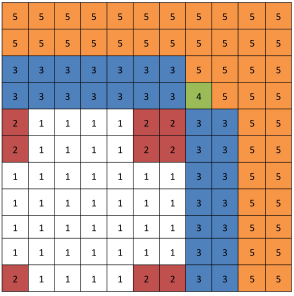
\includegraphics[width=0.4\linewidth]{core}
  \caption{Core Geometry}
  \label{geom}
\end{figure}
\begin{table}[h]
\centering
\begin{tabular}{c c | c c c c}
Region & Group & $D_g$ & $\Sigma_{a,g}$ & $\nu\Sigma_{f,g}$ & $\Sigma_s^{1,2}$ \\ \hline
1 & 1 & 1.255 & 8.252e-3 & 4.602e-3 & 2.533e-2 \\
 & 2 & 2.11e-1 & 1.003e-1 & 1.091e-1 & \\ \hline
2 & 1 & 1.268 & 7.181e-3 & 4.609e-3 & 2.767e-2 \\
 & 2 & 1.902e-1 & 7.047e-2 & 8.675e-2 & \\ \hline
3 & 1 & 1.259 & 8.002e-3 & 4.663e-3 & 2.617e-2 \\
 & 2 & 2.091e-1 & 8.344e-2 & 1.021e-1 & \\ \hline
4 & 1 & 1.259 & 8.002e-3 & 4.663e-3 & 2.617e-2 \\
 & 2 & 2.091e-1 & 7.3324e-2 & 1.021e-1 & \\ \hline
5 & 1 & 1.257 & 6.034e-4 & 0 & 4.754e-2 \\
 & 2 & 1.592e-1 & 1.911e-2 & 0 & 
\end{tabular}
\caption{Reference Material Properties for Benchmark Core}
\label{tab:coremats}
\end{table}
\begin{figure}[H]
\centering
  \begin{subfigure}[b]{0.45 \textwidth}
   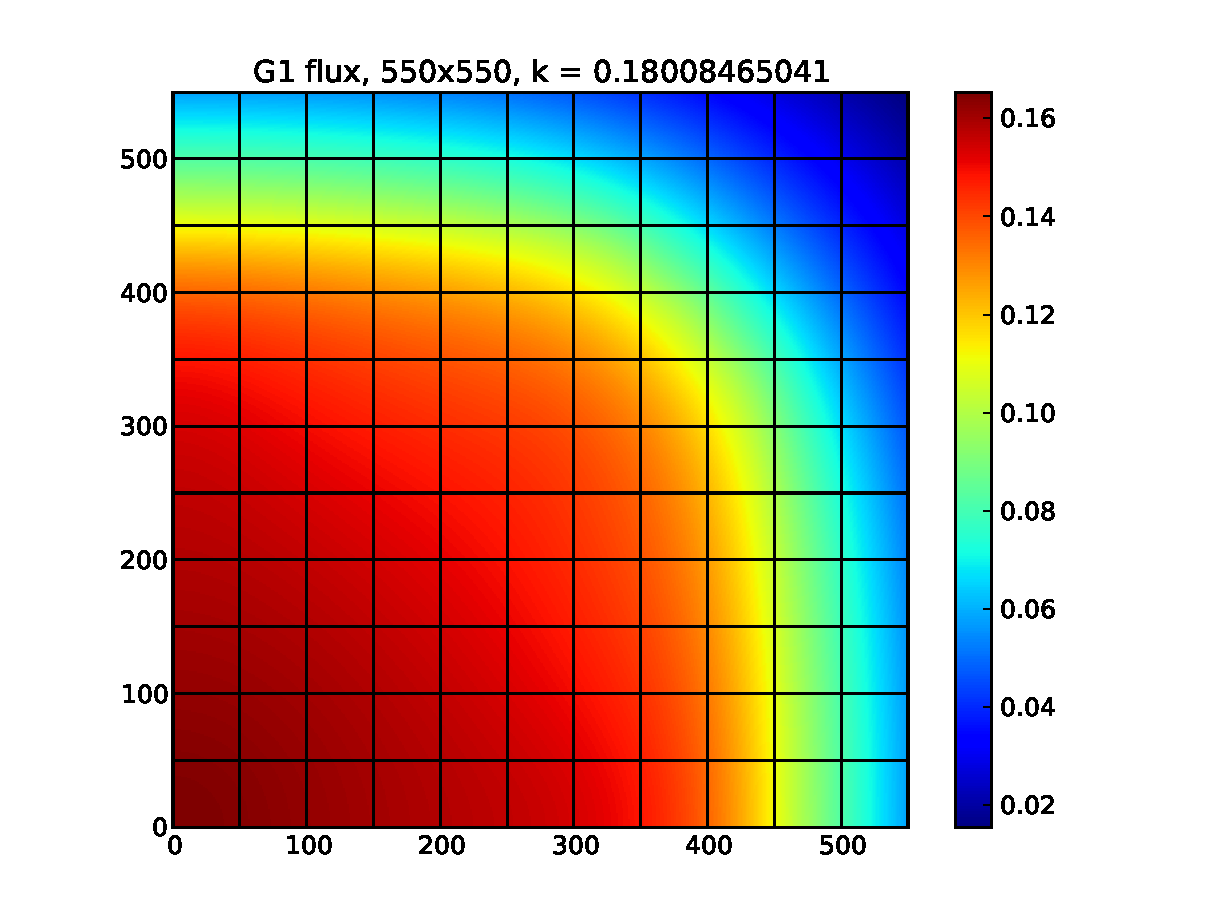
\includegraphics[width=\textwidth]{g1_50_flux}
   \caption{$\phi$, Group 1}
   \label{g1}
  \end{subfigure}
  \begin{subfigure}[b]{0.45 \textwidth}
   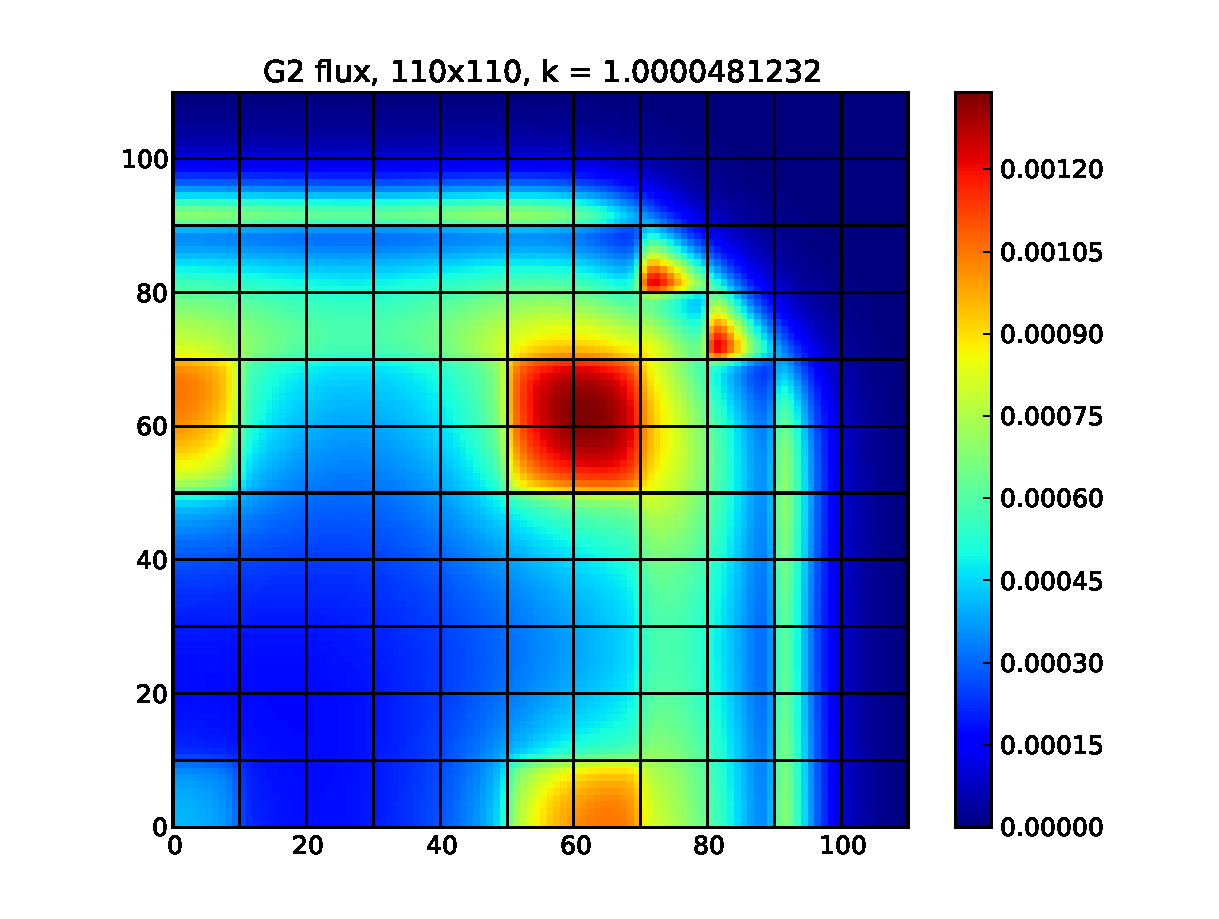
\includegraphics[width=\textwidth]{g2_50_flux}
   \caption{$\phi$, Group 2}
   \label{g2}
  \end{subfigure}
  \caption{Reference Flux Profiles}
  \label{benchflux}
\end{figure}



\section{Fuel Rod Performance}
While the previous codes were designed and written by the author, \bison{} is a professional use code
maintained by Idaho National Laboratory.  The fuel performance simulation used in this work is described
in \cite{cristiansmeared},
and involves an axial-symmetric LWR fuel rodlet, composed of ten uranium dioxide pellets, zirconium-4
cladding, gap, and upper plenum.  The problem is a power ramp-up transient as delineated in Table
\ref{tab:bison power ramp}.  The three uncertain input parameters are distributed in a truncated normal and
are shown in Table \ref{tab:bison dists}.  Note that scaling parameters are used for both grain radius and
reactor power, such that a scaling factor of one is the nominal unperturbed case.
\begin{table}[h]
  \centering
  \begin{tabular}{c|c}
    Time (s) & Linear Power (W/m) \\ \hline
    0 & 0 \\
    1e4 & 3.5e4 \\
    1.5e8 & 3.5e4
  \end{tabular}
  \caption{Linear Power Time Evolution}
  \label{tab:bison power ramp}
\end{table}
\begin{table}[h]
  \centering
  \begin{tabular}{c|c|c}
    Variable & Min. Value & Max. Value \\ \hline
    Grain Radius Scale Factor & 0.4 & 1.5 \\
    Thermal Expansion Coefficient & 9e-6 & 1.1e-5 \\
    Linear Power Scaling Factor & 0.95 & 1.05
  \end{tabular}
  \caption{Fuel Performance Input Distributions}
  \label{tab:bison dists}
\end{table}

The quantity of interest are the stresses on the axial center of the cladding.  The
uncertain parameters used in this test case are the mesoscale grain radius of the fuel, the simulated power
of the reactor surrounding the fuel rod, and the thermal expansion coefficient of the fuel.
